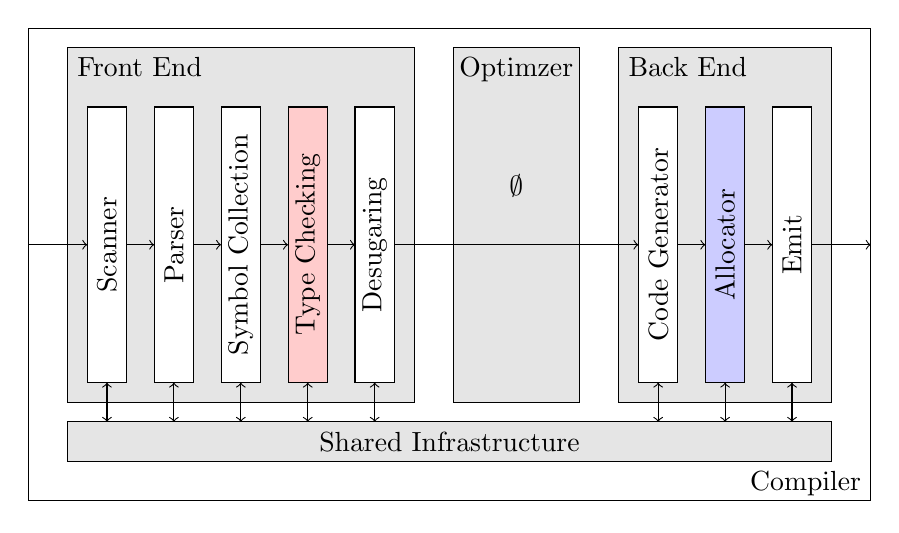
\begin{tikzpicture}
    \draw (0, 0) rectangle ++(10.7, 6) node[anchor=north east, yshift=-5.5cm]{Compiler};
    \filldraw[fill=gray!20] (.5, .5) rectangle ++ (9.7, .5) node[pos=.5]{Shared Infrastructure};
    \filldraw[fill=gray!20] (.5, 1.25) rectangle ++(4.4, 4.5);
    \filldraw[fill=gray!20] (5.4, 1.25) rectangle ++(1.6, 4.5) node[pos=.5, yshift=.5cm]{$\emptyset$};
    \filldraw[fill=gray!20] (7.5, 1.25) rectangle ++(2.7, 4.5);
    \node[anchor=north west] at (.5, 5.75) {Front End};
    \node[anchor=north west] at (5.35, 5.75) {Optimzer};
    \node[anchor=north west] at (7.5, 5.75) {Back End};
    \filldraw[fill=white] (.75, 1.5) rectangle ++(.5, 3.5) node[pos=.5, rotate=90]{Scanner};
    \filldraw[fill=white] (1.6, 1.5) rectangle ++(.5, 3.5) node[pos=.5, rotate=90]{Parser};
    \filldraw[fill=white] (2.45, 1.5) rectangle ++(.5, 3.5) node[pos=.5, rotate=90]{Symbol Collection};
    \filldraw[fill=red!20] (3.3, 1.5) rectangle ++(.5, 3.5) node[pos=.5, rotate=90]{Type Checking};
    \filldraw[fill=white] (4.15, 1.5) rectangle ++(.5, 3.5) node[pos=.5, rotate=90]{Desugaring};
    \filldraw[fill=white] (7.75, 1.5) rectangle ++(.5, 3.5) node[pos=.5, rotate=90]{Code Generator};
    \filldraw[fill=blue!20] (8.6, 1.5) rectangle ++(.5, 3.5) node[pos=.5, rotate=90]{Allocator};
    \filldraw[fill=white] (9.45, 1.5) rectangle ++(.5, 3.5) node[pos=.5, rotate=90]{Emit};
    \draw[->] (0, 3.25) -- ++(0.75, 0);
    \draw[->] (1.25, 3.25) -- ++(0.35, 0);
    \draw[->] (2.1, 3.25) -- ++(0.35, 0);
    \draw[->] (2.95, 3.25) -- ++(0.35, 0);
    \draw[->] (3.8, 3.25) -- ++(0.35, 0);
    \draw[->] (4.65, 3.25) -- ++(3.1, 0);
    \draw[->] (8.25, 3.25) -- ++(0.35, 0);
    \draw[->] (9.1, 3.25) -- ++(0.35, 0);
    \draw[->] (9.95, 3.25) -- ++(0.75, 0);
    \draw[<->] (1, 1) -- ++(0, 0.5);
    \draw[<->] (1.85, 1) -- ++(0, 0.5);
    \draw[<->] (2.7, 1) -- ++(0, 0.5);
    \draw[<->] (3.55, 1) -- ++(0, 0.5);
    \draw[<->] (4.4, 1) -- ++(0, 0.5);
    \draw[<->] (8, 1) -- ++(0, 0.5);
    \draw[<->] (8.85, 1) -- ++(0, 0.5);
    \draw[<->] (9.7, 1) -- ++(0, 0.5);
\end{tikzpicture}